\chapter{Herramienta $\mathtt{SAT\_Solver}$}

\hfil \textit{La esencia de las matemáticas no es hacer las cosas simples complicadas, sino hacer las cosas complicadas simples.}

\hfil \hfil \hfil  Stanley Gudder \\\\

En el presente capítulo se expondrá una herramienta para resolver el famoso problema de satisfacibilidad o más conocido como el problema $SAT$. Dicha herramienta se basará en la aproximación algebraica presentada en los capítulos anteriores, mostrando así una de sus más relevantes aplicaciones. \\

Se describirán los distintos módulos de la herramienta, detallando los procesos más relevantes. Es importante destacar que los cálculos llevados a cabo por el programa se dividen principalmente en dos etapas:
\begin{enumerate}
\item Preprocesado del fichero de entrada.
\item Decisión por saturación con la regla de independencia.
\end{enumerate}

Finalmente, se realizará un análisis de eficiencia de la herramienta, durante el cual se detectaron ciertas ``fugas de tiempo''. Estas posibles mejoras se implementarán también dando lugar a una primera versión del \texttt{SAT-Solver}.

\section{Fichero de entrada y el formato \texttt{DIMACS}}
Previo a la descripción del formato \texttt{DIMACS} es necesaria una definición formal de qué es la forma normal conjuntiva. Con este objetivo se verán antes dos definiciones de la lógica proposicional.

\defn Un literal es una fórmula atómica o su negación. Se dice que un literal es \textit{positivo} si se trata de un átomo y \textit{negativo} si es la negación de un átomo.\\

Por ejemplo, $p_1$, $p_2$ ó $\neg p_1$ son literales.

\defn Una cláusula es una disyunción de literales. En otras palabras, es una colección finita de literales que es verdadera si alguno de ellos lo es. \\

Por ejemplo, $p_1 \vee p_2$ ó $p_1 \vee \neg p_2 \vee \neg p_3$ son cláusulas. Ya se está en condiciones de definir la forma normal conjuntiva.

\defn Dada una fórmula proposicional $F$ se dice que está en forma normal conjuntiva si se trata de una conjunción de cláusulas. \\

Con respecto al problema de satisfacibilidad es importante saber el que criterio debe cumplir una fórmula en forma normal conjuntiva para ser verdadera. Esta condición es que en todas sus cláusulas debe haber al menos un literal que sea verdadero.\\

Otra propiedad que se debe conocer sobre la forma normal conjuntiva es que dada cualquier fórmula proposicional existe otra equivalente en forma normal conjuntiva. 

El algoritmo que la calcula es el siguiente \cite{apuntes} :

\begin{center}
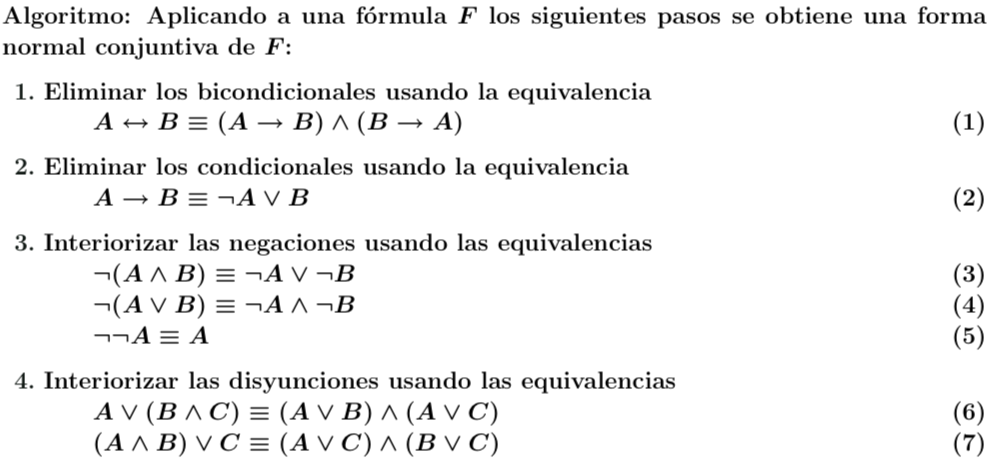
\includegraphics[scale=0.45]{imagenes/algfnc}
\end{center}

Como ya se ha comentado, se pretende presentar la herramienta a una competición, por tanto, debe cumplir ciertos requisitos para poder participar. El principal y más importante es que las instancias del problema $SAT$ que debe resolver vienen dadas en lo que se denomina el formato \texttt{DIMACS}. Un ejemplo de cómo se codificaría la fórmula $(p_1 \vee \neg p_5 \vee p_4)\wedge(\neg p_1 \vee p_5 \vee p_3 \vee p_4) \wedge (\neg p_3 \vee \neg p_4)$ en formato \texttt{DIMACS} es

\begin{table}[h]
\centering
\label{ej:dimacs}
\begin{tabular}{l}
\texttt{c} \\\\
\texttt{c start with comments} \\\\
\texttt{c} \\\\
\texttt{c}  \\\\
\texttt{p cnf 5 3} \\\\
\texttt{1 -5 4 0} \\\\
\texttt{-1 5 3 4 0} \\\\
\texttt{-3 -4 0}
%{\Large \texttt{c} }\\\\
%{\Large \texttt{c start with comments}} \\\\
%{\Large \texttt{c}} \\\\
%{\Large \texttt{c}}  \\\\
%{\Large \texttt{p cnf 5 3}} \\\\
%{\Large \texttt{1 -5 4 0}} \\\\
%{\Large \texttt{-1 5 3 4 0}} \\\\
%{\Large \texttt{-3 -4 0}}
\end{tabular}
\end{table}

\newpage

Dicho formato es una estandarización simplificada de la forma normal conjuntiva de una fórmula. Las instancias serán archivos de texto (\texttt{.txt} o \texttt{.cnf}) con la siguiente estructura:

\begin{enumerate}
\item En primer lugar, se encuentran las líneas de comentarios. Se identifican gracias a que están encabezadas por la letra \texttt{c}. En el ejemplo, son las cuatro primeras líneas.
\item En segundo lugar, hay una línea distinguida que indica las propiedades de la fórmula como, por ejemplo, que está en forma normal conjuntiva (\texttt{cnf}). El primer número que aparece indica el mayor índice de una variable proposicional (normalmente coincide con el número de variables proposicionales) mientras que el segundo cuántas cláusulas. 
\item Finalmente, en cada línea se encuentra codificada una cláusula distinta según las siguientes indicaciones:
\begin{itemize}
\item Cada número entero representa un literal.
\item El signo del número, positivo o negativo, indica si dicho literal es positivo o negativo, respectivamente.
\item El final de la cláusula se codifica con un 0.
\end{itemize} 
\end{enumerate}

\newpage
\section{Preprocesado}

Las funciones que intervienen en el preprocesado transforman un archivo \texttt{.txt} ó \texttt{.cnf} en formato \texttt{DIMACS} en el conjunto de polinomios que les corresponde según la función $\pi$. A continuación, se presentan estas funciones.

\entrada{Preprocesado}

Con el objetivo de comprender las dimensiones del problema con el que se trabaja, se muestra a continuación un ejemplo del uso de la función \texttt{dimacsAPolinomios} en el fichero (no trivial) de menor tamaño:

\begin{code}
> dimacsAPolinomios "exDIMACS/medium/exampleSat0.txt"
(fromList [x1x10x38+x1x10+x1x38+x1+x10x38+x10+x38,
x10x48x59+x10x59+x48x59+x59+1,x10x76x88+x10x76+x76x88+x76+1,
x14x34x50+x14x34+x14x50+x14+1,x14x59x87+x59x87+1,
x16x28x84+x16x28+x16x84+x16+x28x84+x28+x84,x18x55x64+x55x64+1,
x19x3x30+x19x3+1,x19x57x93+x19x57+x19x93+x19+1,x2x21x98+x21x98+1,
x20x4x80+x20x80+1,x23x7x72+x23x72+1,x28x60x8+x28x60+1,x3x35x96+x35x96+1,
x31x42x89+x31x42+x42x89+x42+1,x31x5x97+x5x97+1,x35x47x64+x35x47+1,
x35x48x58+x35x48+x35x58+x35+1,x36x56x78+x36x78+x56x78+x78+1,
x4x65x94+x4x65+x4x94+x4+1,x44x76x78+x44x78+1,x48x52x63+x48x63+1,
x52x94x99+x52x94+x94x99+x94+1,x55x63x90+x55x63+1,
x59x75x9+x59x75+x59x9+x59+x75x9+x75+x9,x65x83x89+x65x83+x65x89+x65+1,
x68x84x88+x68x88+1,x75x86x89+x75x86+1,x81x88x92+x81x88+1,1],
[x1,x10,x14,x16,x18,x19,x2,x20,x21,x23,x28,x3,x30,x31,x34,x35,x36,x38,
x4,x42,x44,x47,x48,x5,x50,x52,x55,x56,x57,x58,x59,x60,x63,x64,x65,x68,
x7,x72,x75,x76,x78,x8,x80,x81,x83,x84,x86,x87,x88,x89,x9,x90,x92,x93,
x94,x96,x97,x98,x99])
\end{code}

\newpage
\section{Saturación}

Una vez que se tiene el conjunto de polinomios basta saturar dicho conjunto usando la regla de independencia. Las funciones encargadas de realizar este proceso son: \texttt{omiteVariableKB} y \texttt{saturaKB}. El módulo en el que se implementan estas se llama \texttt{Saturacion}.

\entrada{Saturacion}

Y así queda implementada una primera versión de la herramienta.

\newpage
\section{Análisis de la herramienta}

En esta sección se probará la herramienta con instancias del problema, con el objetivo de detectar cotas de eficiencia. Dichos ejemplos se han obtenido de dos fuentes:
\begin{itemize}
\item[•] Construidos manualmente (almacenados en el directorio \texttt{easy})
\item[•] Truncando (o no) tres ejemplos de la web de la \href{http://www.satcompetition.org}{SAT Competition}.
\end{itemize}

 Las instancias se almacenan en el directorio \texttt{exDIMACS}, organizadas en carpetas según su longitud.

\subsection{Directorio \texttt{easy}}
Este directorio contiene cuatro ejemplos muy sencillos, de hecho, las fórmulas que codifican sólo  tienen 2 variables ($p$ y $q$). El objetivo de estos ejemplos es servir como test para comprobar que el funcionamiento de la herramienta es el deseado.

\subsubsection{Ejemplo 1}

El archivo se llama \texttt{example1.txt}:
\begin{codigo}
c example 1 
c 
c f = (p ∨ q)
c
p cnf 2 1 
1 2 0
\end{codigo}

Y codifica la fórmula:
$$(p \vee q)$$

La ejecución en máquina es:
\begin{code}
>>> satSolver "exDIMACS/easy/example1.txt"
True
(0.00 secs, 586,368 bytes)
\end{code}
\subsubsection{Ejemplo 2}
El archivo se llama \texttt{example2.txt}:
\begin{codigo}
c example 2
c 
c f = (p ∨ q) ∧ (¬p ∨ q)
c
p cnf 2 2
1 2 0
-1 2 0
\end{codigo}

Y codifica la fórmula:
$$(p \vee q) \wedge (\neg p \vee q)$$

La ejecución en máquina es:
\begin{code}
>>> satSolver "exDIMACS/easy/example2.txt"
True
(0.00 secs, 792,784 bytes)
\end{code}
\subsubsection{Ejemplo 3}
El archivo se llama \texttt{example3.txt}:
\begin{codigo}
c example 3
c 
c f = (p ∨ q) ∧ (¬p ∨ q) ∧ (p ∨ ¬q)
c
p cnf 2 3
1 2 0
-1 2 0
1 -2 0
\end{codigo}

Y codifica la fórmula:
$$(p \vee q)\wedge (\neg p \vee q)\wedge ( p \vee \neg q)$$

La ejecución en máquina es:
\begin{code}
>>> satSolver "exDIMACS/easy/example3.txt"
True
(0.00 secs, 1,047,600 bytes)
\end{code}
\subsubsection{Ejemplo 4}
El archivo se llama \texttt{example4.txt}:
\begin{codigo}
c example 4
c 
c f = (p ∨ q) ∧ (¬p ∨ q) ∧ (p ∨ ¬q) ∧ (¬p ∨ ¬q)
c
p cnf 2 4
1 2 0
-1 2 0
1 -2 0
-1 -2 0
\end{codigo}

Y codifica la fórmula:
$$(p \vee q)\wedge (\neg p \vee q)\wedge ( p \vee \neg q)\wedge (\neg p \vee \neg q)$$

La ejecución en máquina es:
\begin{code}
>>> satSolver "exDIMACS/easy/example4.txt"
False
(0.01 secs, 1,361,672 bytes)
\end{code}

\subsection{Directorio \texttt{medium}}
Tras comprobar que la herramienta responde de la forma deseada con los ejemplos anteriores, conviene probar su eficiencia. Para ello, se construye una batería de ejemplos truncando el archivo \texttt{sat100.cnf} del directorio \texttt{hard}. \\

Al ser conjuntos de cláusulas contenidas en un conjunto de cláusulas satisfacible son también satisfacibles y por tanto, el resultado de usar la herramienta debe ser \texttt{True}.\\

Únicamente se tratarán los tres primeros ejemplos ya que el resto no se ejecuta en un tiempo razonable.

\subsubsection{Ejemplo 0}
El archivo se llama \texttt{exampleSat0} y codifica una fórmula en forma normal conjuntiva con 30 cláusulas en las que intervienen hasta 59 variables distintas. \\ 

Destacar que tanto en este ejemplo como en los próximos, en cada cláusula habrá exactamente 3 literales.

La ejecución en máquina es:
\begin{code}
>>> satSolver "exDIMACS/medium/exampleSat0.txt"
True
(0.02 secs, 10,307,480 bytes)
\end{code}

\newpage

El archivo es:

\begin{codigo}
c 
c    clause length = 3 
c
p cnf 59 30
30 -19 -3 0
89 31 -42 0
1 10 38 0
2 -21 -98 0
36 56 -78 0
14 -59 -87 0
89 -75 -86 0
-20 -80 4 0
-63 90 -55 0
59 75 9 0
-5 31 -97 0
48 -35 58 0
28 84 16 0
65 -4 94 0
-72 -23 7 0
18 -64 -55 0
-96 3 -35 0
89 -65 83 0
8 -60 -28 0
34 50 -14 0
64 -47 -35 0
-19 57 93 0
52 99 -94 0
-59 10 48 0
-78 -44 76 0
-63 -48 52 0
-88 84 -68 0
10 88 -76 0
92 -81 -88 0
\end{codigo}

\subsubsection{Ejemplo 5}
El archivo se llama \texttt{exampleSat1.txt} y codifica una fórmula satisfacible con 91 cláusulas y 82 variables. Por razones de espacio se omitirá mostar el archivo. La ejecución en máquina es:
\begin{code}
>>> satSolver "exDIMACS/medium/exampleSat1.txt"
True
(5.87 secs, 2,122,138,840 bytes)
\end{code}

\subsubsection{Ejemplo 6}
El archivo se llama \texttt{exampleSat2.txt} y codifica una fórmula satisfacible de mayor tamaño que la anterior, de hecho, la contiene. Por razones de espacio se omitirá mostar el archivo. La ejecución en máquina es:
\begin{code}
>>> satSolver "exDIMACS/medium/exampleSat2.txt"
True
(139.13 secs, 34,754,329,424 bytes)
\end{code}

\subsection{Directorio \texttt{hard}}

En este directorio se encuentras tres archivos \texttt{.cnf} que son tres ejemplos oficiales de instancias dadas por la organización de la competición $SAT$ en la que se pretende participar.

\subsubsection{Archivo \texttt{sat100.cnf}}
Este ejemplo consta de 100 variables en 430 cláusulas. La fórmula es satisfacible pero tiempo de ejecución sobrepasa la hora.
\subsubsection{Archivo \texttt{sat250.cnf}}
Este ejemplo consta de 250 variables en 1065 cláusulas. La fórmula es satisfacible aunque el tiempo de ejecución excede la hora.
\subsubsection{Archivo \texttt{unsat250.cnf}}
Este ejemplo consta de 250 variables en 1065 cláusulas. La fórmula es insatisfacible y la ejecución queda:
\begin{code}
>>> satSolver "exDIMACS/hard/unsat250.cnf"
False
(0.05 secs, 34,873,832 bytes)
\end{code}

\subsection{Heurísticas}
Ya en el ejemplo 5, el tiempo de ejecución es demasiado alto. Sin embargo, en el ejemplo 6 y posteriores (exceptuando \texttt{unsat250.cnf}) el coste en tiempo excede lo razonable, por lo que se pone de manifiesto la necesidad de una mejora en la implementación.\\

Tras diversas pruebas, la mejora que se ha implementado se debe al hecho observado de que aunque el resultado tras saturar permanezca invariante si se cambia el orden de las variables a omitir, el tiempo de ejecución sí cambia.\\

A raíz de esto se probarán experimentalmente varias heurísticas; y en base a estos experimentos, se escogerá la que tenga mejores resultados. Es importante tener en cuenta que no es seguro que el orden escogido sea el óptimo ya que nos basamos en un criterio absolutamente empírico.\\

Se define el módulo \texttt{Heuristicas}, en el que se implementarán dichas heurísticas.

\entrada{Heuristicas}

\newpage

Quedando la solución del ejemplo 5:

\begin{code}
>>> satSolver heuristicaOrdMon "exDIMACS/medium/exampleSat1.txt"
True
(5.82 secs, 2,122,150,944 bytes)
>>> satSolver heuristicaFrecuencia "exDIMACS/medium/exampleSat1.txt"
True
(0.24 secs, 62,955,680 bytes)
>>> satSolver heuristicaFrecRev "exDIMACS/medium/exampleSat1.txt"
True
(7.08 secs, 3,372,336,472 bytes)
\end{code}

Mientras que la del ejemplo 6:

\begin{code}
>>> satSolver heuristicaOrdMon "exDIMACS/medium/exampleSat2.txt"
True
(137.98 secs, 34,754,335,488 bytes)
>>> satSolver heuristicaFrecuencia "exDIMACS/medium/exampleSat2.txt"
True
(0.30 secs, 92,607,744 bytes)
>>> satSolver heuristicaFrecRev "exDIMACS/medium/exampleSat2.txt"
Interrupted.
\end{code}

Tras varios minutos de espera queda patente que la tercera heurística no es eficiente.  La segunda (\texttt{heuristicaFrecuencia}) con el ejemplo 7 y con \texttt{unsat250.cnf} da los siguientes resultados:

\begin{code}
>>> satSolver heuristicaFrecuencia "exDIMACS/medium/exampleSat3.txt"
True
(5.87 secs, 2,317,863,248 bytes)
>>> satSolver heuristicaFrecuencia "exDIMACS/hard/unsat250.cnf"
False
(0.06 secs, 34,872,144 bytes)
\end{code}

En función de estos resultados, la heurística escogida es \texttt{heuristicaFrecuencia}. Sin embargo, el tiempo sigue siendo demasiado alto si se quiere resolver el ejemplo 8 o algunas de las dos instancias satisfacibles del directorio \texttt{hard}.